\section{Grundlegende Arten von qualitätssichernden Maßnahmen}

Eines der wichtigsten Ziele bei der Softwareentwicklung ist es, Risiken zu minimieren (vgl.~\cite[7]{Wed09c}).\\
Dieses Ziel kann erreicht werden, wenn die Einhaltung \textit{jeder} \textbf{Qualitätsforderung} durch mindestens eine Maßnahme sichergestellt wird.\\

\noindent
Spezielle Systematiken können dabei helfen, geeignete Maßnahmen aus einer Vielzahl von \textbf{Qualitätsmaßnahmen}  auszuwählen (s. Abbildung~\ref{fig:systematik qualitätsmaßnahmen}).

\begin{figure}
    \centering
    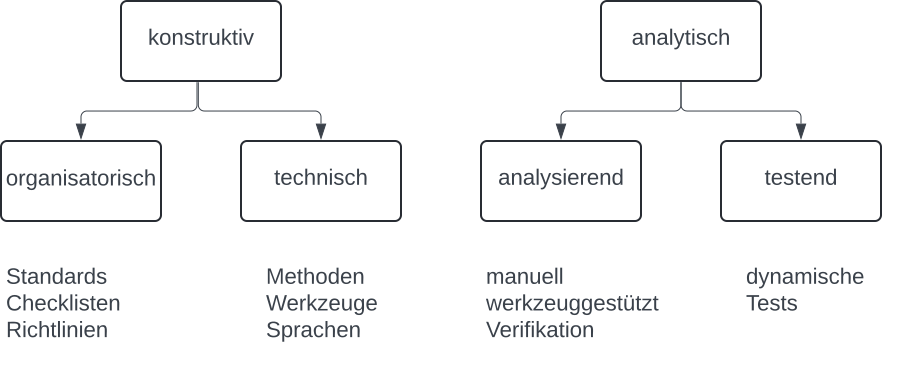
\includegraphics[scale=0.4]{part four/Typen von Qualitätsmaßnahmen/img/systematik qualitätsmaßnahmen}
    \caption{Systematik der Typen von Qualitätsmaßnahmen. (Quelle: in Anlehnung an~\cite[Abb. 2.1, 8]{Wed09c})}
    \label{fig:systematik qualitätsmaßnahmen}
\end{figure}

\subsection*{Konstruktiv und analytisch}
\textbf{Konstruktive Maßnahmen} sollen die Entstehung von Defekten, die Fehler verursachen, verhindern.\\
\textbf{Analytische Maßnahmen} werden eingesetzt, um entstandene Defekte zu entdecken, damit sie anschließend beseitigt werden können.

\subsection*{Konstruktive Maßnahmen - organisatorische Maßnahmen}
Bei \textbf{konstruktiven Verfahren} werden \textbf{organisatorische} und \textbf{technische Verfahren} unterschieden.

\begin{itemize}
    \item \textbf{Organisatorische Verfahren}: Richtlinien, Checklisten, Standards. Beispiel: Vorlage für User Storys, die alle im Projekt verwenden müssen.
    \item \textbf{technische Verfahren}: technische Qualitätsmaßnahmen wie Methoden, Werkzeuge, Einsatz anderer Programmiersprachen. Beispiel: Einsatz von Tools zur Einhaltung von Coding-Standards.
\end{itemize}

\noindent
\textbf{Konstruktive Maßnahmen} sind vor allem Gegenstand des Projektmanagements, weshalb \textit{Wedemann} sie nicht weitere thematisiert (vgl.~\cite[9]{Wed09c}).


\subsection*{Analytische Maßnahmen}
bei \textbf{analytischen Maßnahmen} werden \textbf{analysierende} und \textbf{testende Maßnahmen} unterschieden.

\begin{itemize}
    \item \textbf{analysierende Maßnahmen}: Prüfgegenstand wird systematisch untersucht, ohne ihn in Funktion zu nehmen.\\
    Hierzu werden \textbf{manuelle} und \textbf{werkzeuggestützte Maßnahmen} sowie die \textbf{Verifikation} als analysierende Maßnahmen verwendet:
    \begin{itemize}
        \item \textbf{manuelle Maßnahmen}: Menschen \textit{lesen} und \textit{analysieren} Prüfgegenstände: Bspw. indem User Storys gegengelesen werden, oder ein objektorientierter Entwurf überprüft wird
        \item \textbf{werkzeuggestützte Maßnahmen}: Analysen werden maschinell von Software durchgeführt: Bspw. das Überprüfen im Quellcode auf typische Defekte (leere catch-Blöcke)
        \item \textbf{Verifikation}: Nachweis der Richtigkeit von Quellcode durch mathematische Verfahren\footnote{
        \textit{Wedemann} weist darauf hin, dass dieses Verfahren keine allgemeine Relevanz hat und nur auf speziellen Gebieten eingesetzt wird: Es wird in der Praxis zumeist durch das werkzeuggestützte Verfahren der \textit{abstrakten Interpretation} abgelöst (vgl.~\cite[9]{Wed09c}; s. a. Abschnitt~\ref{subsec:abstrakte-interpretation})
        }
    \end{itemize}
    \item  \textbf{testende Maßnahmen}: Prüfgegenstand wird in Betrieb genommen, das \textbf{beobachtete Verhalten} wird mit dem \textbf{spezifizierten Verhalten} verglichen (\textbf{dynamischer Test})
\end{itemize}

\begin{tcolorbox}
    Der \textbf{dynamische Test} ist die minimale Art der Qualitätssicherung: Nur, wenn eine Software auch ausgeführt wurde, kann man davon ausgehen, dass sie funktioniert (vgl.~\cite[9]{Wed09c})
\end{tcolorbox}
\vspace{2mm}

\noindent
Der Test ist nicht immer die effektivste Form, Defekte zu verhindern: Lesen des Quelltexts oder Werkzeuge eignen sich oft sehr gut: Ein Test kann außerdem nicht bestimmte Eigenschaften des Quellcodes sicherstellen, wie die \textbf{Wartbarkeit}.\\
``Dokumente und Modelle lassen sich garnicht testen`` (\cite[10]{Wed09c}).
